% !TEX root = ../../../main/aws_chabauty.tex
\newpage
\subsection{Lecture 4}

	\begin{figure}[!ht]
	\centering
	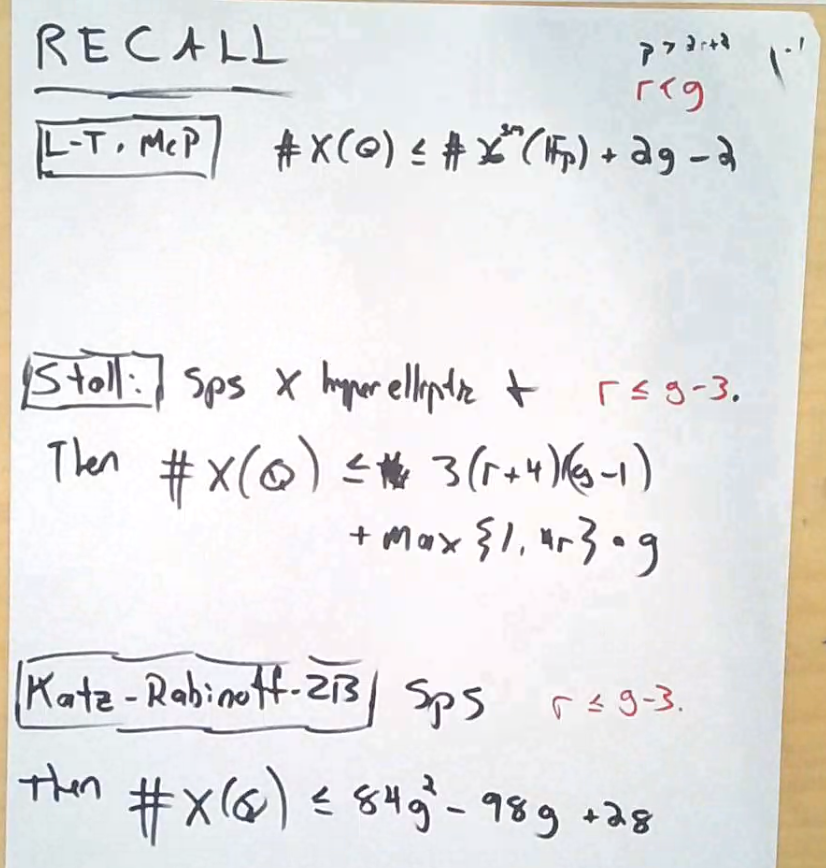
\includegraphics[width=0.5\textwidth]{../images/im34.png}
	\end{figure}

	\begin{figure}[!ht]
	\centering
	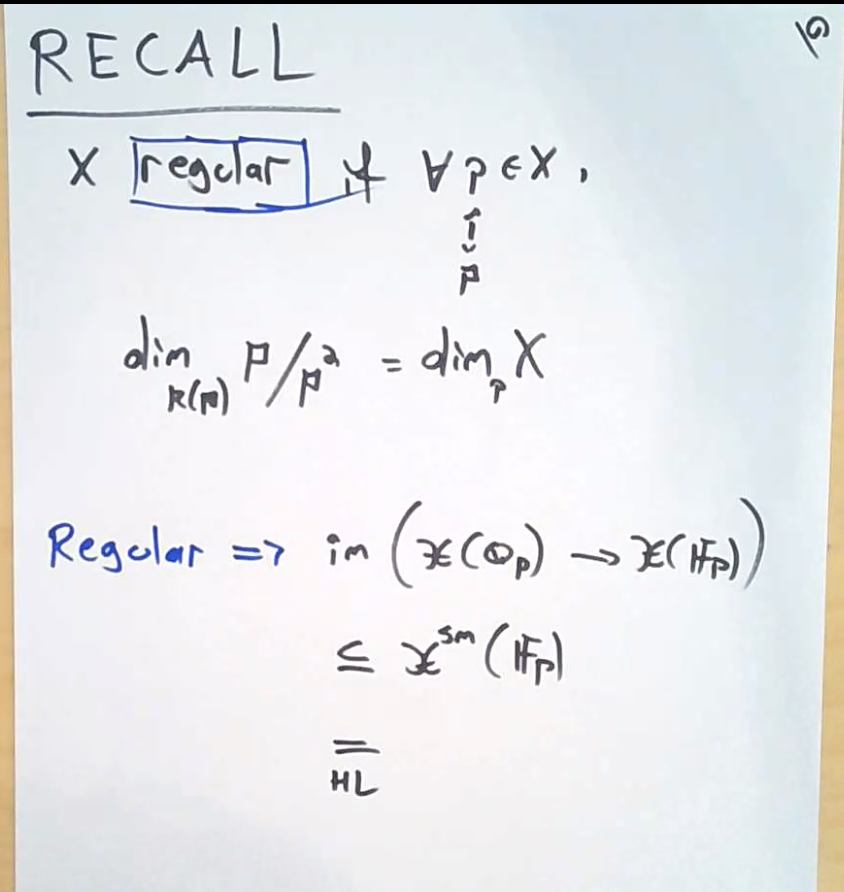
\includegraphics[width=0.5\textwidth]{../images/im35.png}
	\end{figure}

Problem: $\fX^{\text{sm}}(\F_p)$ is unbounded. $xyz= p(x^3+y^3+z^3)$. 

	\begin{figure}[!ht]
	\centering
	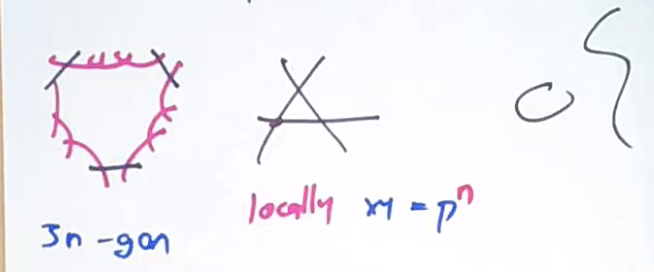
\includegraphics[width=0.5\textwidth]{../images/im36.png}
	\end{figure}

Stoll

\begin{itemize}
\item Work of non-regular model
\item cont. chains of $\P^1$'s
\item then $\fX(\F_p)$ is bounded via $p$ and $g$
\end{itemize}


Problem: Setup and local analysis is hard.


Main Tool: (KRZB)

Systematic use of Berkovich and tropical geometry

Setup, 2 types of $\int$'s
	\[
	\int_{\text{abelian}} + \int_{\text{Berk.-Coleman}}
	\]
The abelian integral comes from Lie $J$ and ????. The Berk.-Coleman integral is more computable and not equal to $\int_{\text{Ab}}$. The difference between the two is linear in $\omega$. The difference factors through Trop $T$, where $T$ is 
	\[
	\begin{tikzcd}
	& T \subseteq & \\
	A & \subseteq \tilde{J} \arrow[two heads]{d} \arrow{r} & J^? \\
	& A \text{ good red}
	\end{tikzcd}
	\]

Local Analysis:

Potential then on $X^\text{an}$.


``Global Step''

``Combinatorial optimization for sections of ``Tropical Canonical bundle''''

Tay version:

$|K \Gamma| \ni D$, bound for the min \# of things for which witness $D \sim K_P$.


Time travel to AWS 2007.

The Gelfand spectrum
$M(R)= \{ R \ma{|\cdot|} \R\}$ set of bounded multi. seminorms 

There is a map $M(R) \to \R$ given by $|\cdot| \mapsto |f|$. 

If $x \in M(R), f \in R$, write ``$f(x):= |f|$''. 


\begin{ex}
Let $\Q_p\{t\} = \sum_{i=0}^\infty a_i t^i$, where $a_i \in \Qp$ with $|a_i| \to 0$. Now$M(\Qp\{t\}) \supseteq \text{max spec } \Qp\{t\} \in x \in \ov{\Z}_p \subseteq \ov{\Q}_p$. 

	\begin{figure}[!ht]
	\centering
	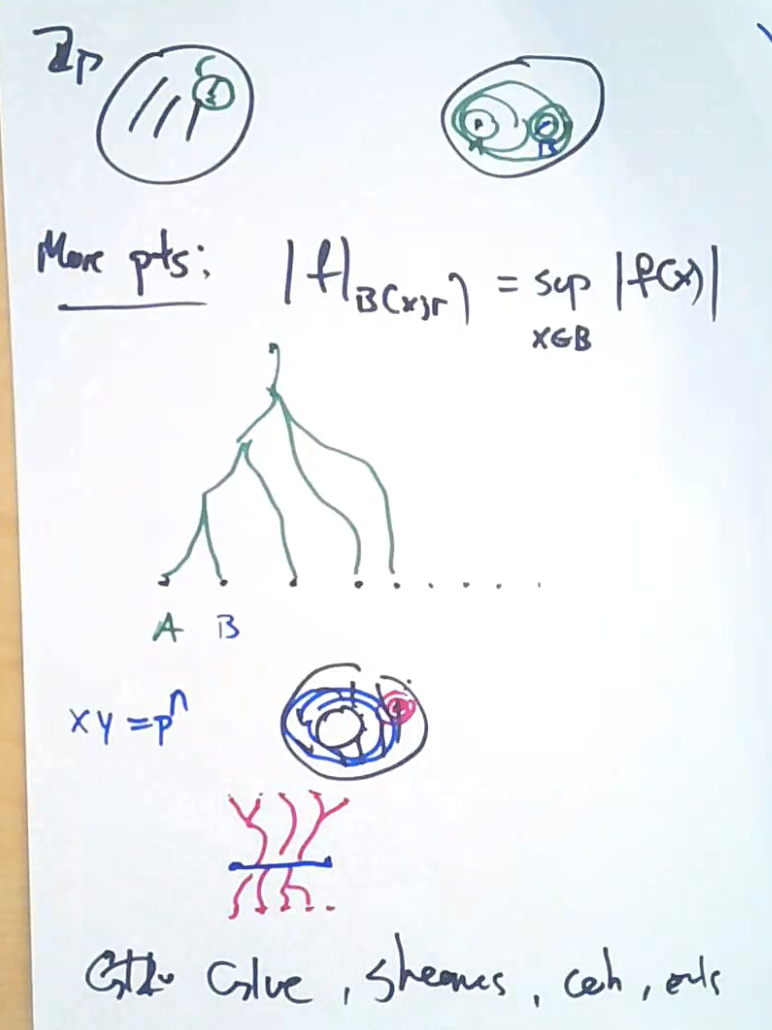
\includegraphics[width=0.5\textwidth]{../images/im37.png}
	\end{figure}

Max points: $|f|_{B(x|f)}= \sup_{x \in B} |f(x)|$
\end{ex}


Fundamental Theorem of Tropical Geometry:

Baker-Payne-Rabinoff
Berkovich, Thuiller

$\fX/\Z_p$ s.stable

$xyz= p(x^3+y^3+z^3)$.


	\begin{figure}[!ht]
	\centering
	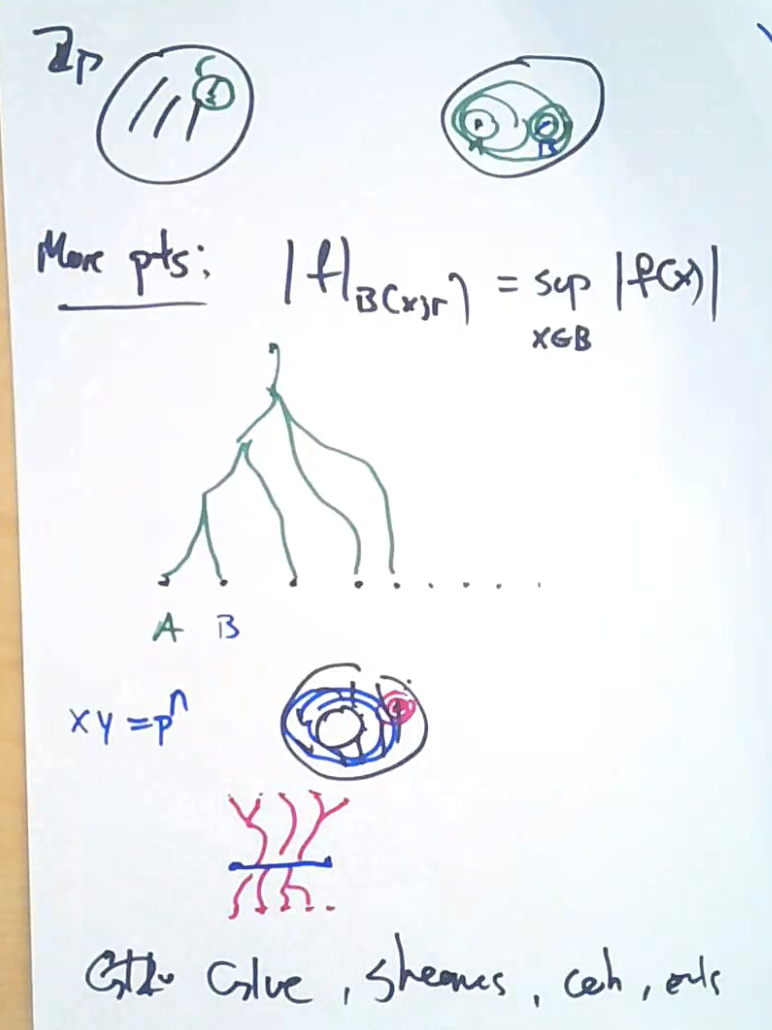
\includegraphics[width=0.5\textwidth]{../images/im37.png}
	\end{figure}

Potential Thm:

$\fX \ma{\text{an }f} \P^1$

$F(x)= - \log|f(x)|$, $F \big|_P$ is $P \big|_W$ linear


\begin{thm}
$\tau_* \div f= \div F:= \sum (\text{slope newton poly at }P) [P]$
\end{thm}


\begin{ex}
$f(x;y;z):= [x;z]$
$\div f= [0 \colon \xi_o \colon 1]= -([1 \colon \xi_0 \colon 0] + \cdots)$
$?????????$


% Rabinoff Utah survey paper photo

	\begin{figure}[!ht]
	\centering
	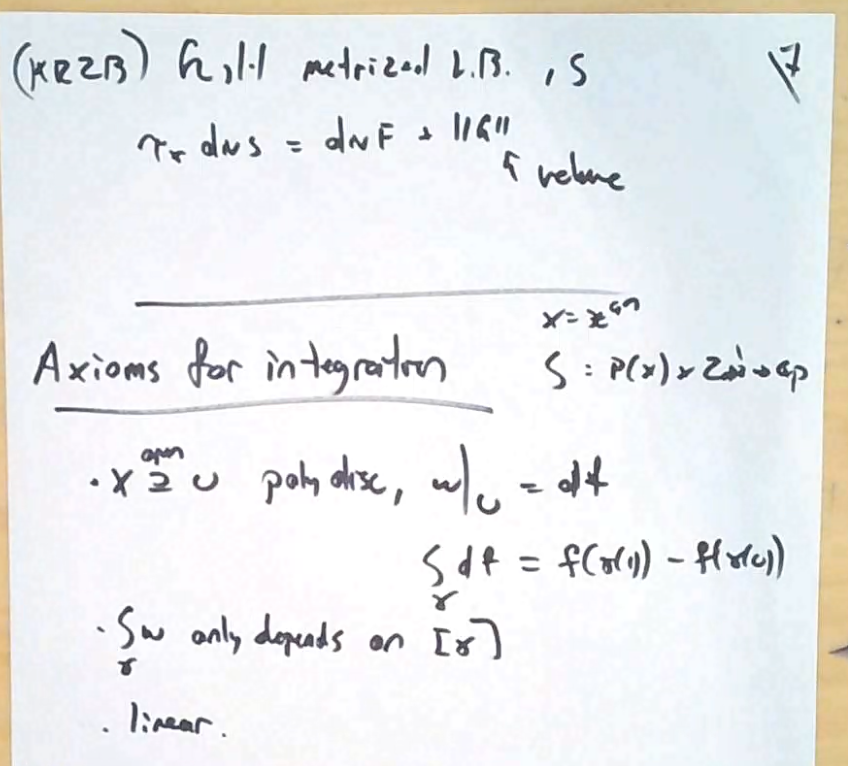
\includegraphics[width=0.5\textwidth]{../images/im40.png}
	\end{figure}
\end{ex}


	\begin{figure}[!ht]
	\centering
	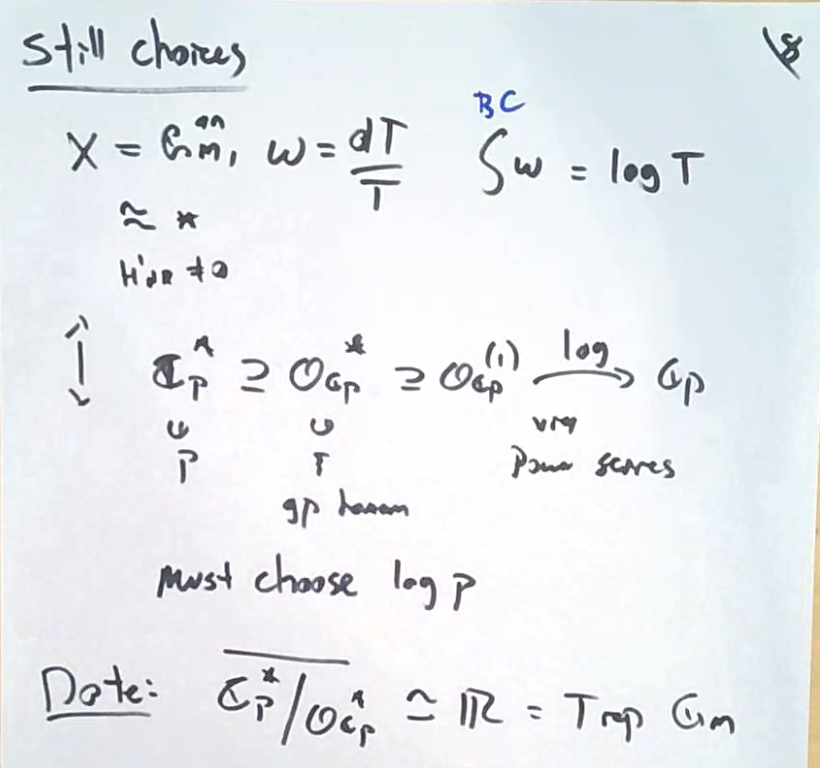
\includegraphics[width=0.5\textwidth]{../images/im41.png}
	\end{figure}

	\begin{figure}[!ht]
	\centering
	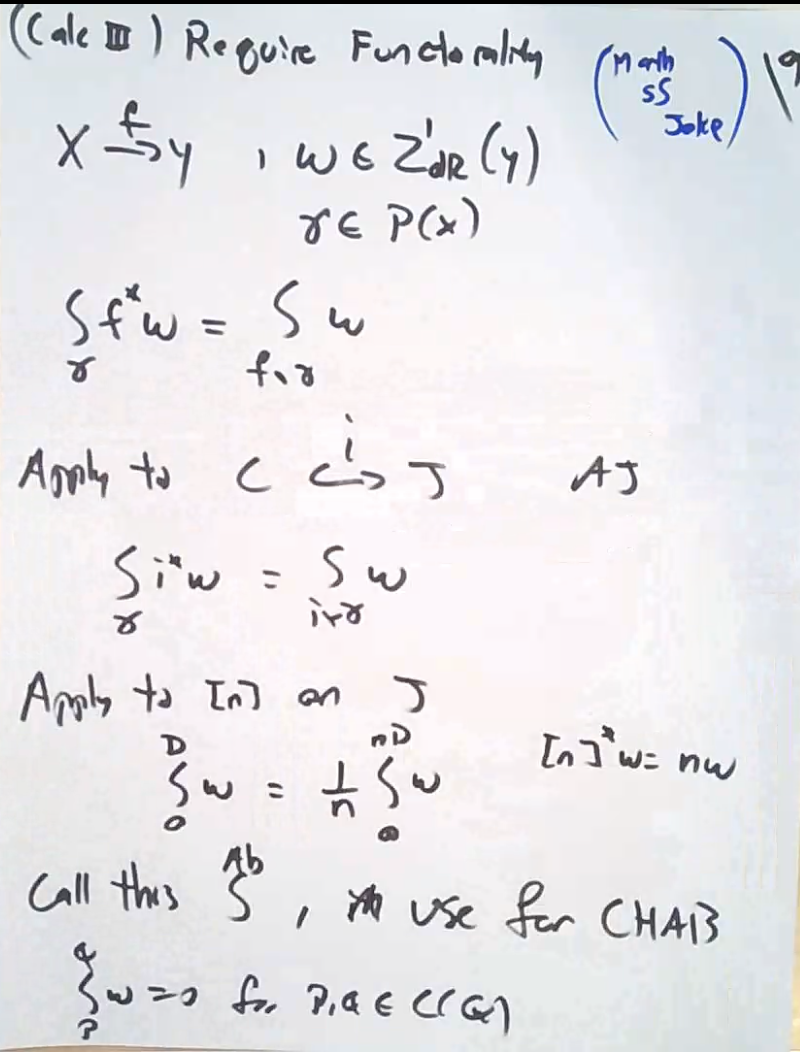
\includegraphics[width=0.5\textwidth]{../images/im42.png}
	\end{figure}

	\begin{figure}[!ht]
	\centering
	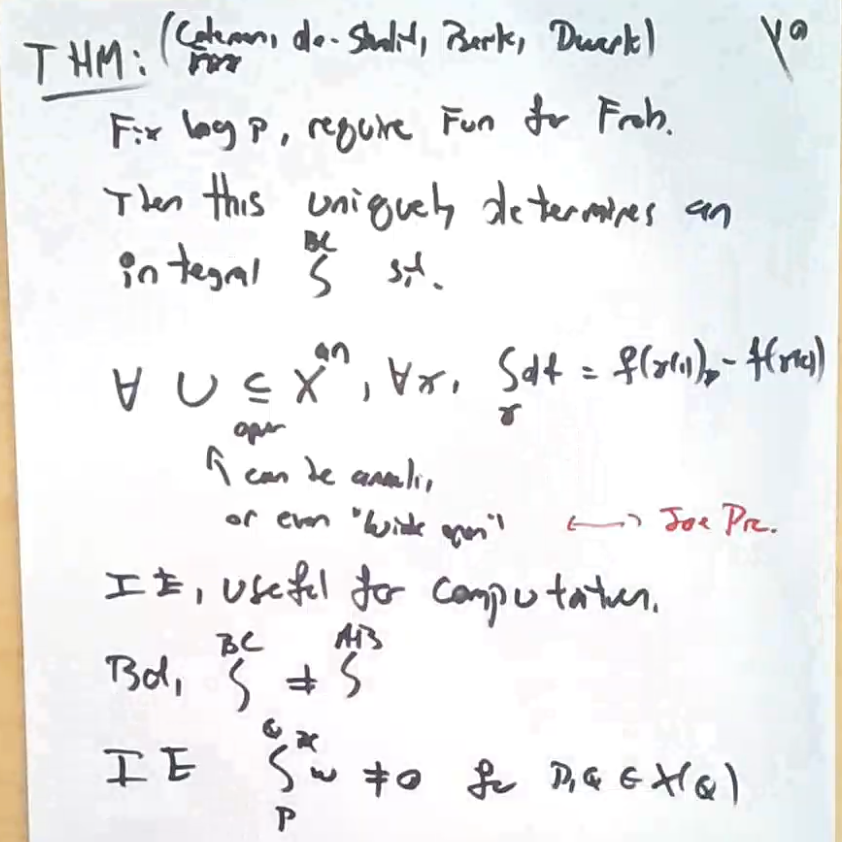
\includegraphics[width=0.5\textwidth]{../images/im43.png}
	\end{figure}


	\begin{figure}[!ht]
	\centering
	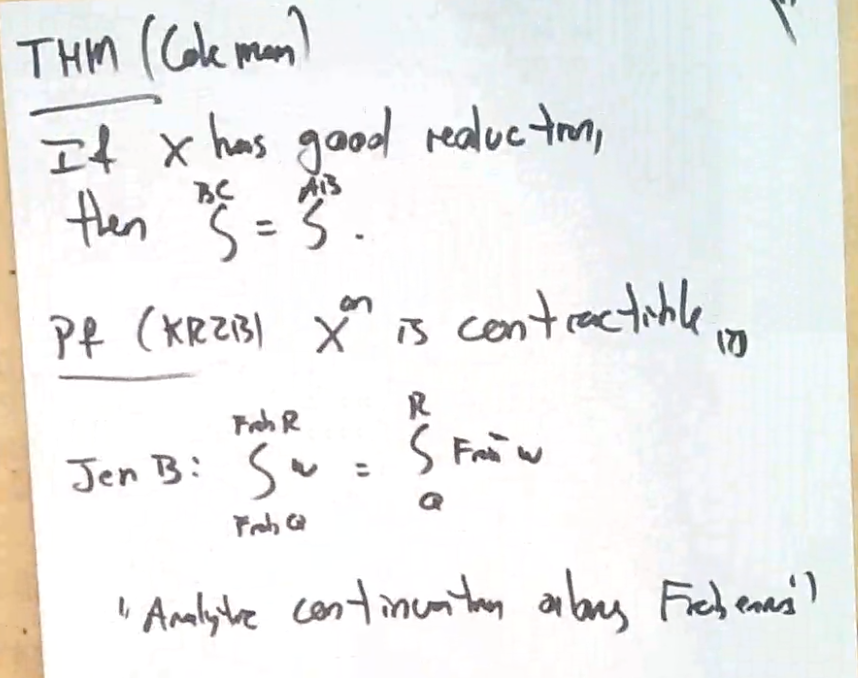
\includegraphics[width=0.5\textwidth]{../images/im44.png}
	\end{figure}

	\begin{figure}[!ht]
	\centering
	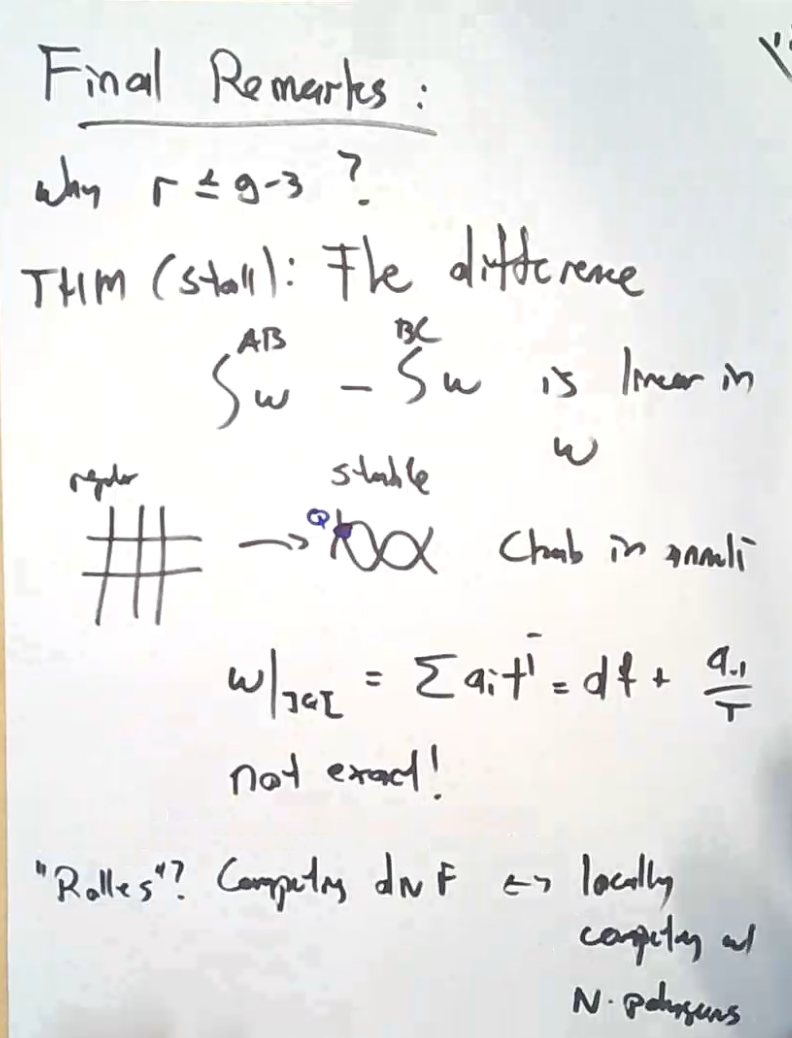
\includegraphics[width=0.5\textwidth]{../images/im45.png}
	\end{figure}


























